% AUTO-GENERATED by scripts/build_paper_artifacts.py. DO NOT EDIT BY HAND.
\begin{figure*}[t]
\centering
\begin{minipage}[b]{0.49\linewidth}\centering
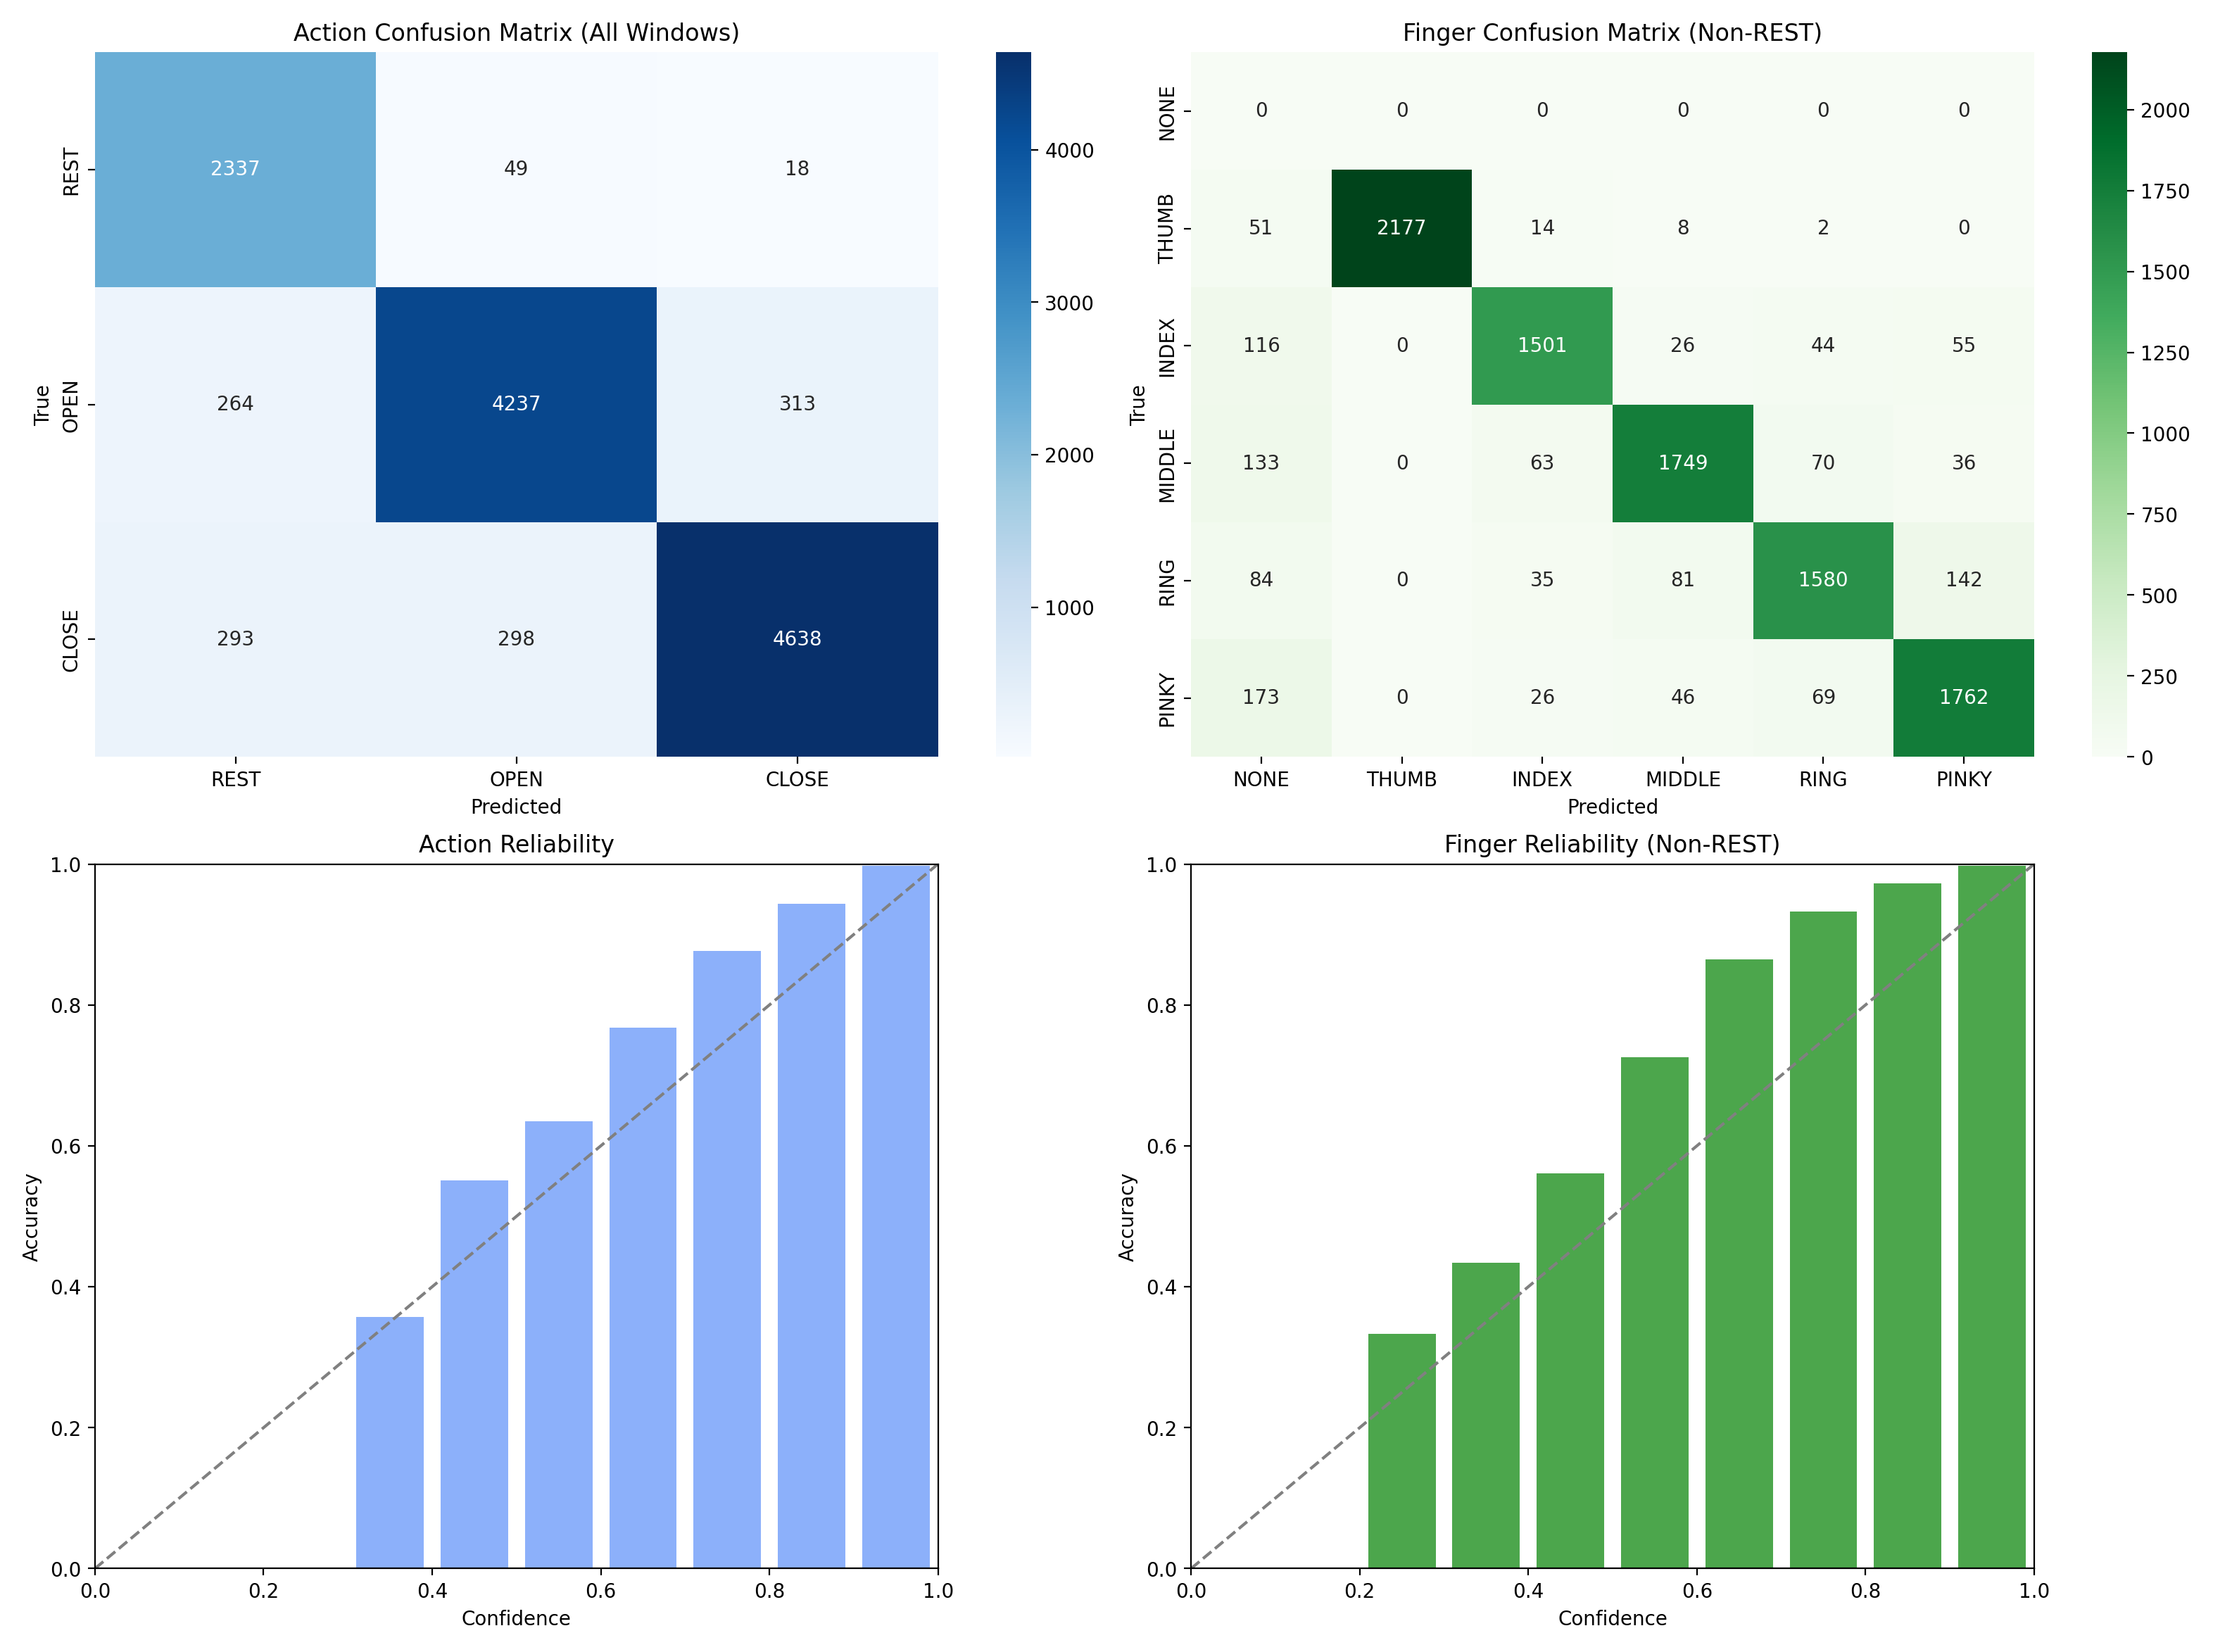
\includegraphics[width=\linewidth]{../paper_figures/2-M16_combined_20260319_081200_pruned_rest_events_0_1_2_20260319_075520__mc_eval.png}
\\\footnotesize (a) Step~3c reliability/calibration summary, including action and finger confusion matrices (2-M16).
\end{minipage}
\begin{minipage}[b]{0.49\linewidth}\centering
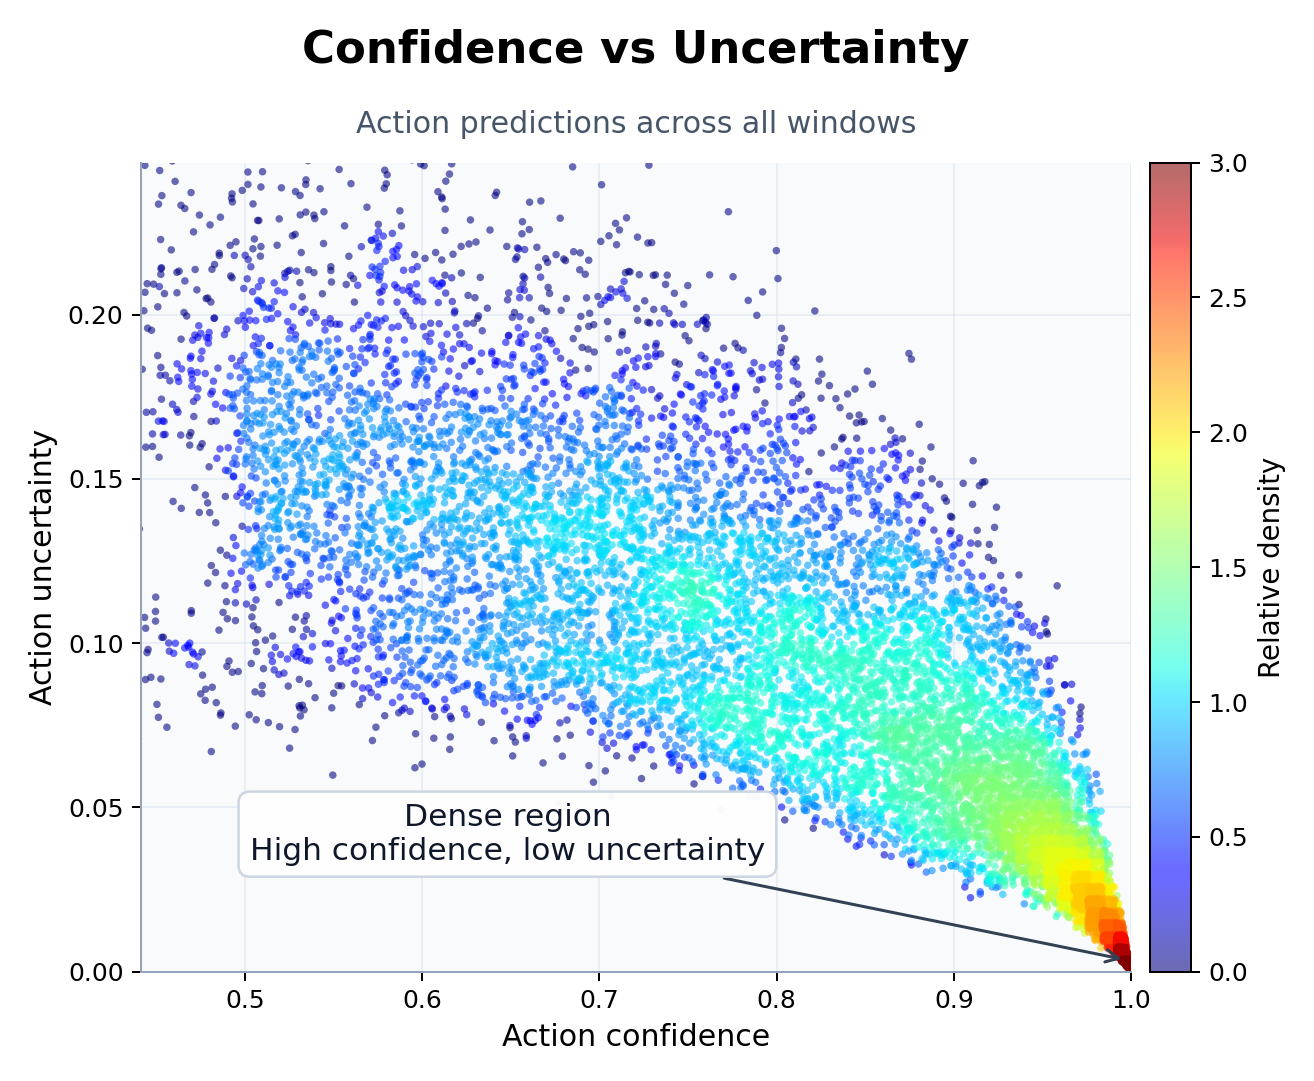
\includegraphics[width=\linewidth]{../paper_figures/2-M16_combined_20260319_081200_pruned_rest_events_0_1_2_20260319_075520__mc_scatter.png}
\\\footnotesize (b) Supporting MC-dropout confidence--uncertainty view (2-M16).
\end{minipage}
\caption{Representative Step~3c evaluation outputs for the featured 2-M16 run. The reliability/calibration panel includes action and finger confusion matrices, while the confidence--uncertainty panel summarizes MC-dropout behavior across windows.}
\label{fig:featured-evaluation}
\end{figure*}

\begin{figure}[t]
\centering
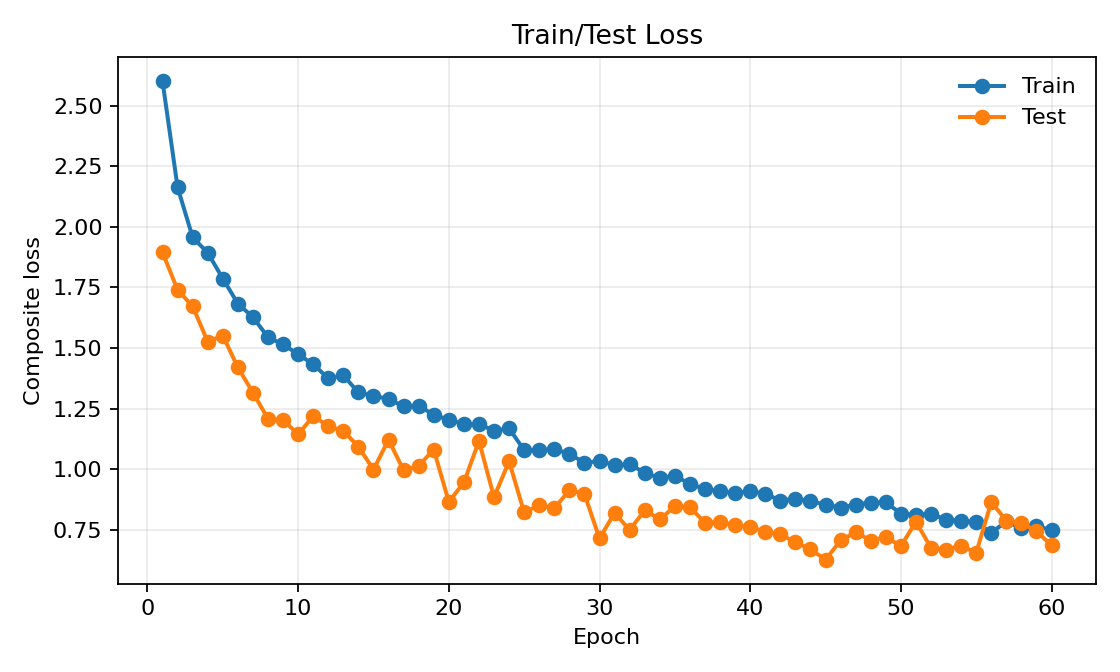
\includegraphics[width=\linewidth]{../paper_figures/2-M16_combined_20260319_081200_pruned_rest_events_0_1_2_20260319_075520__loss_curve.png}
\caption{Additional training-dynamics validation for the featured recipe: train/test composite loss by epoch (featured recipe rerun recorded history). The curve is generated only from recorded per-epoch history and is not reconstructed from final metrics.}
\label{fig:featured-loss-curve}
\end{figure}

